\section{Muhammad Tomy Nur Maulidy(1174031)}
\subsection{Point Polyline dan Polygon}
\begin{enumerate}
	\item 
	\lstinputlisting{src/1174031/2/soal1.py}
	\begin{figure}[H]
		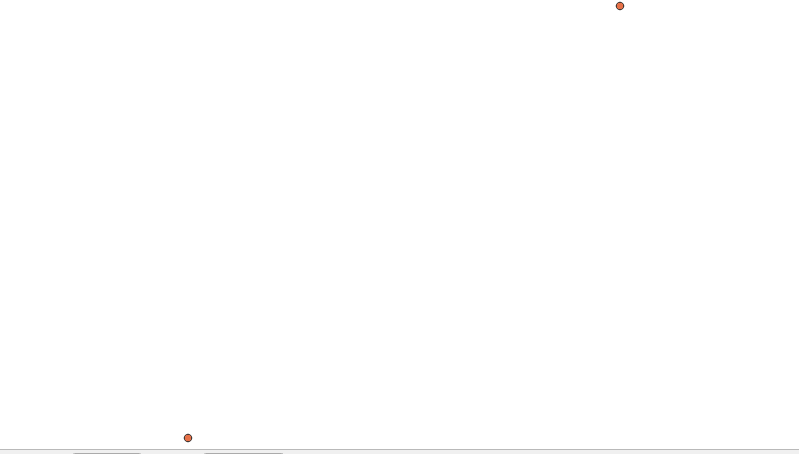
\includegraphics[width=12cm]{figures/1174031/2/hasil1.PNG}
		\centering
		\caption{Point}
	\end{figure}
	
	\item 
	\lstinputlisting{src/1174031/2/soal2.py}
	\begin{figure}[H]
		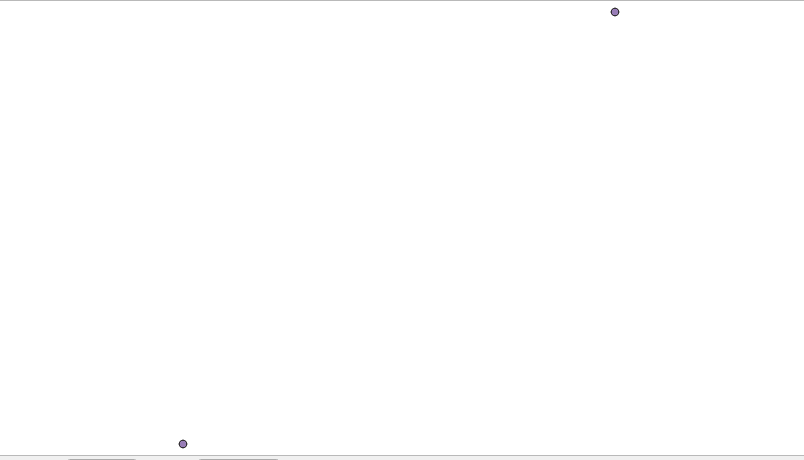
\includegraphics[width=12cm]{figures/1174031/2/hasil2.PNG}
		\centering
		\caption{Point}
	\end{figure}
	
	\item 
	\lstinputlisting{src/1174031/2/soal3.py}
	\begin{figure}[H]
		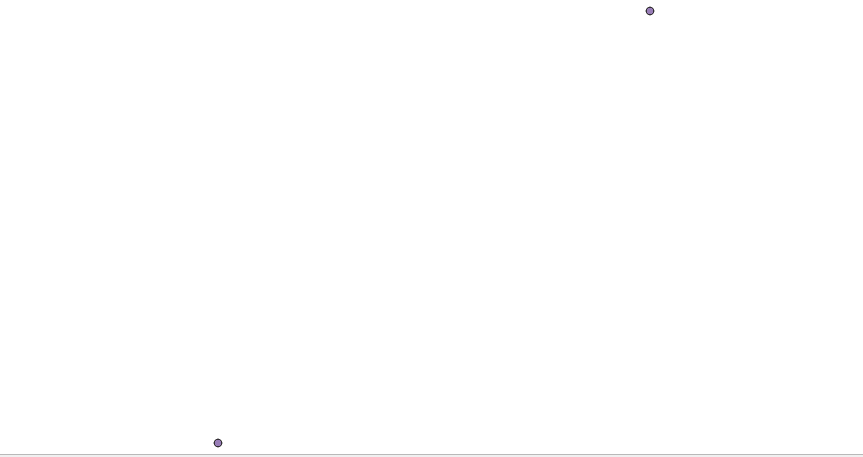
\includegraphics[width=12cm]{figures/1174031/2/hasil3.PNG}
		\centering
		\caption{Point}
	\end{figure}
	
	\item 
	\lstinputlisting{src/1174031/2/soal4.py}
	\begin{figure}[H]
		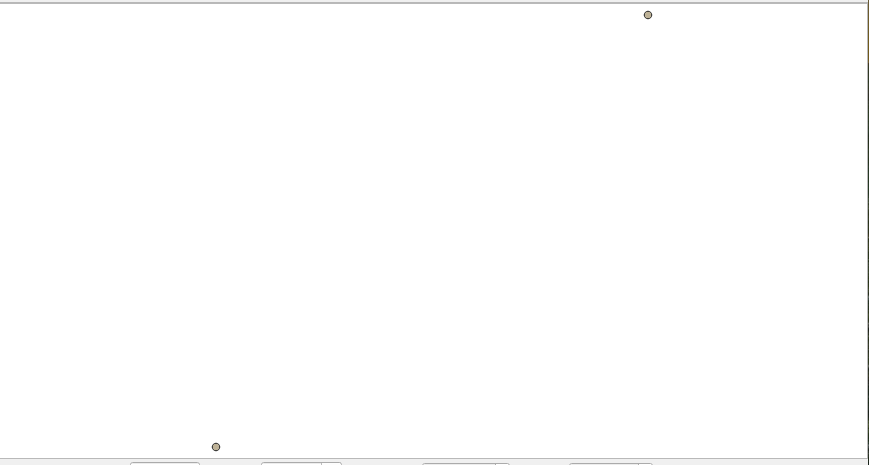
\includegraphics[width=12cm]{figures/1174031/2/hasil4.PNG}
		\centering
		\caption{Point}
	\end{figure}
	
	\item 
	\lstinputlisting{src/1174031/2/soal5.py}
	\begin{figure}[H]
		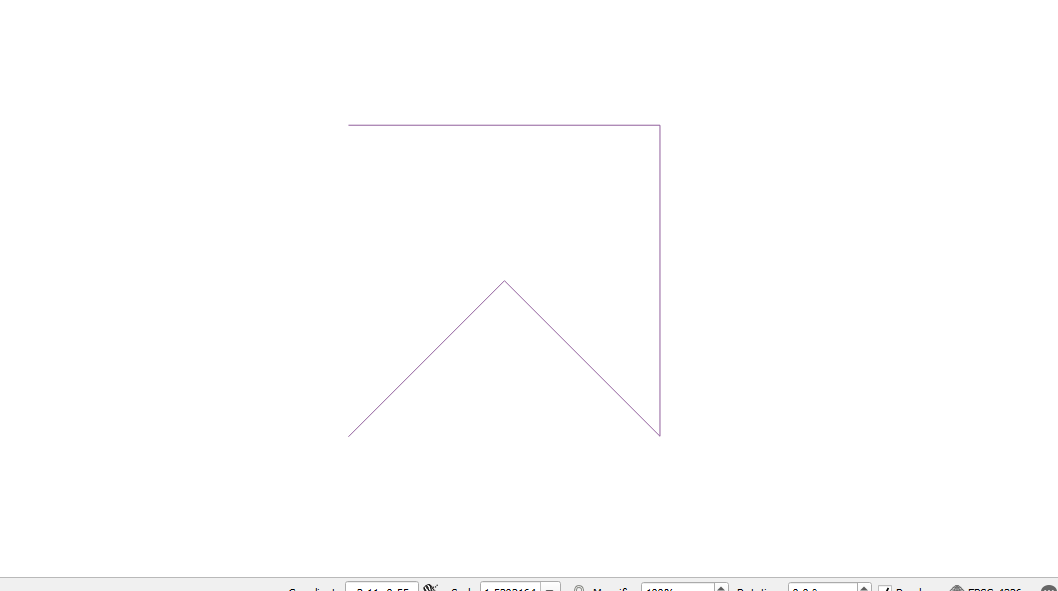
\includegraphics[width=12cm]{figures/1174031/2/hasil5.PNG}
		\centering
		\caption{Polyline}
	\end{figure}
	
	\item 
	\lstinputlisting{src/1174031/2/soal6.py}
	\begin{figure}[H]
		
\includegraphics[width=12cm]{figures/1174031/2/hasil6.PNG}
		\centering
		\caption{Poligon}
	\end{figure}
	
	\item 
	\lstinputlisting{src/1174031/2/soal7.py}
	\begin{figure}[H]
		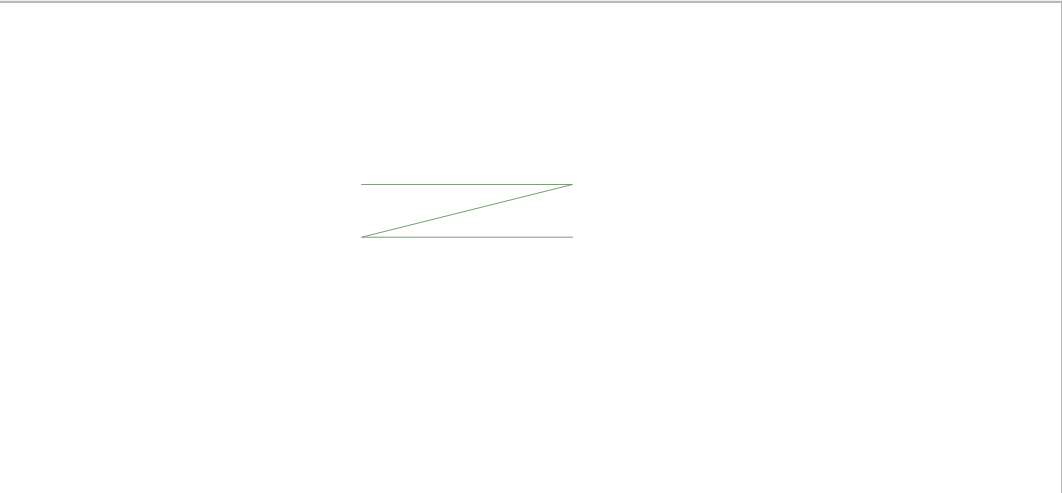
\includegraphics[width=12cm]{figures/1174031/2/hasil7.PNG}
		\centering
		\caption{Polygon}
	\end{figure}
	
	\item 
	\lstinputlisting{src/1174031/2/soal8.py}
	\begin{figure}[H]
		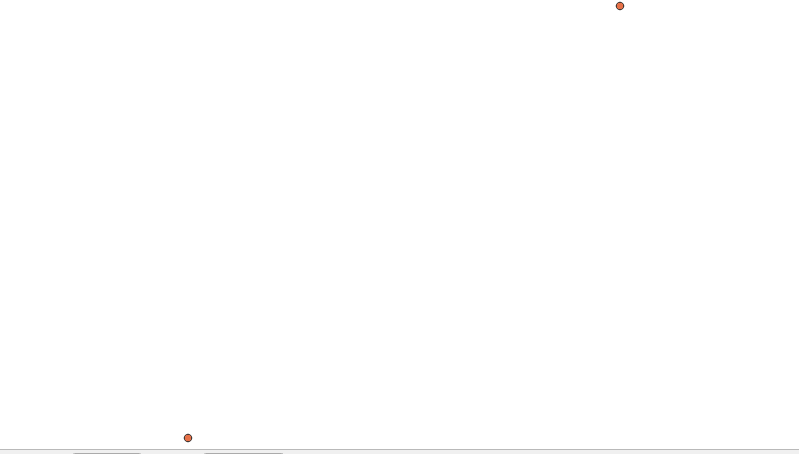
\includegraphics[width=12cm]{figures/1174031/2/hasil1.PNG}
		\centering
		\caption{Polygon}
	\end{figure}
	
	\item 
	\lstinputlisting{src/1174031/2/soal9.py}
	\begin{figure}[H]
		
\includegraphics[width=12cm]{figures/1174031/2/hasil9.PNG}
		\centering
		\caption{Polygon}
	\end{figure}
	
	\item 
	\lstinputlisting{src/1174031/2/soal10.py}
	\begin{figure}[H]
		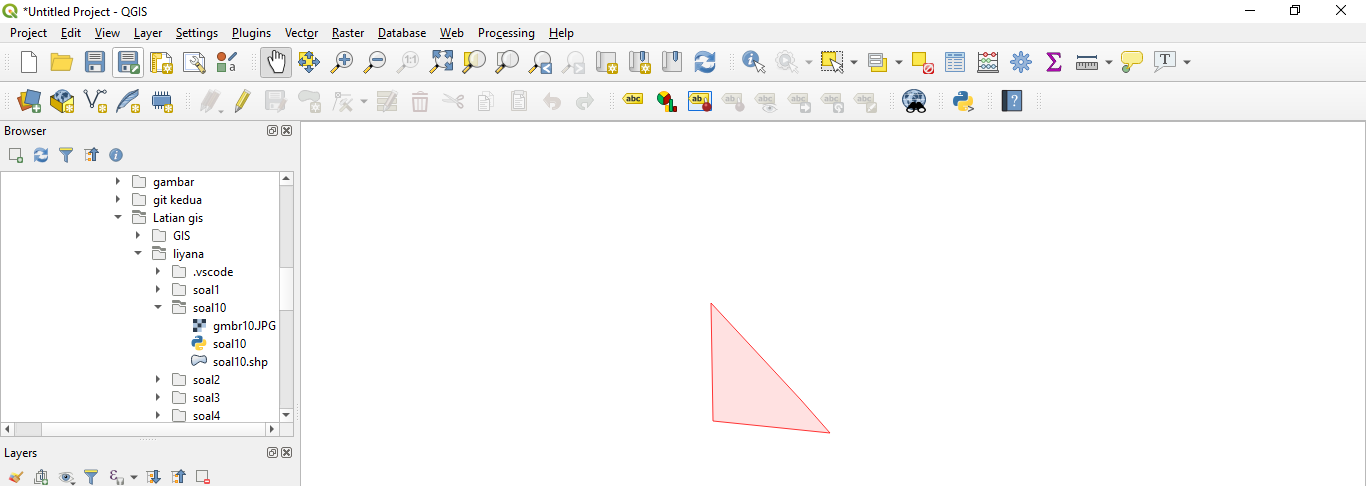
\includegraphics[width=12cm]{figures/1174031/2/hasil10.PNG}
		\centering
		\caption{Hasil mod saya yaitu 7 jadi yang saya kerjakan segitiga siku-siku , Polygon}
	\end{figure}	
\end{enumerate}

\subsection{Link}
\href{https://youtu.be/URVWarQ8wtY}{Youtube}